\section{Financial Report}

The following pages show a sample financial report. Note that it consists of two parts: the \textbf{Income Statement}, which is a record of all the money that's flowed into and out of the club for the past financial year, and the \textbf{Statement of Finanacial Performance}, which summarizes how much money the club has right now. The following terms are used:

\textbf{Income:} This is any money that the club receives through the actions of its members. Examples of income sources include membership fees, fundraisers, tickets to events, sales of assets, \etc. In the sample income statement, income includes membership fees, interest from our savings account, door sales from Buckets of Dice as well as two smaller conventions (Minicon 1 \& 2), and money from an auction of some old assets.

\textbf{Receivables:} The difference between income and receivables is something complex and accounting-y. In SAGA's case, the main receivables are grants from the UCSA.

\textbf{Expenses:} This is any money that you spend. This should be relatively straightforward.

\textbf{Current Assets:} These are assets that we expect to spend or use up by the end of the financial year. In SAGA's case this mainly includes petty cash and our everyday banking account.

\textbf{Non-current Assets:} These are assets that we don't expect to spend or use up by the end of the financial year. In SAGA's case this includes all of our games and our savings account.

\textbf{Liabilities:} These are things that we've resolved to pay, but haven't paid yet. An example of this could be if we owe someone money, or if we've written a cheque but the recipient hasn't cashed it yet. We shouldn't generally have liabilities.

\textbf{Accrued income and expenses:} This is for money that we're owed, or that we owe people. For example:

\begin{itemize}
  \item If the UCSA has awarded you a grant, but hasn't paid you the money yet (accrued income)
  \item If you owe someone money but it hasn't come out of the account yet (accrued expenses)
\end{itemize}

\textbf{Equity:} This is our net worth, calculated as assets minus liabilities.

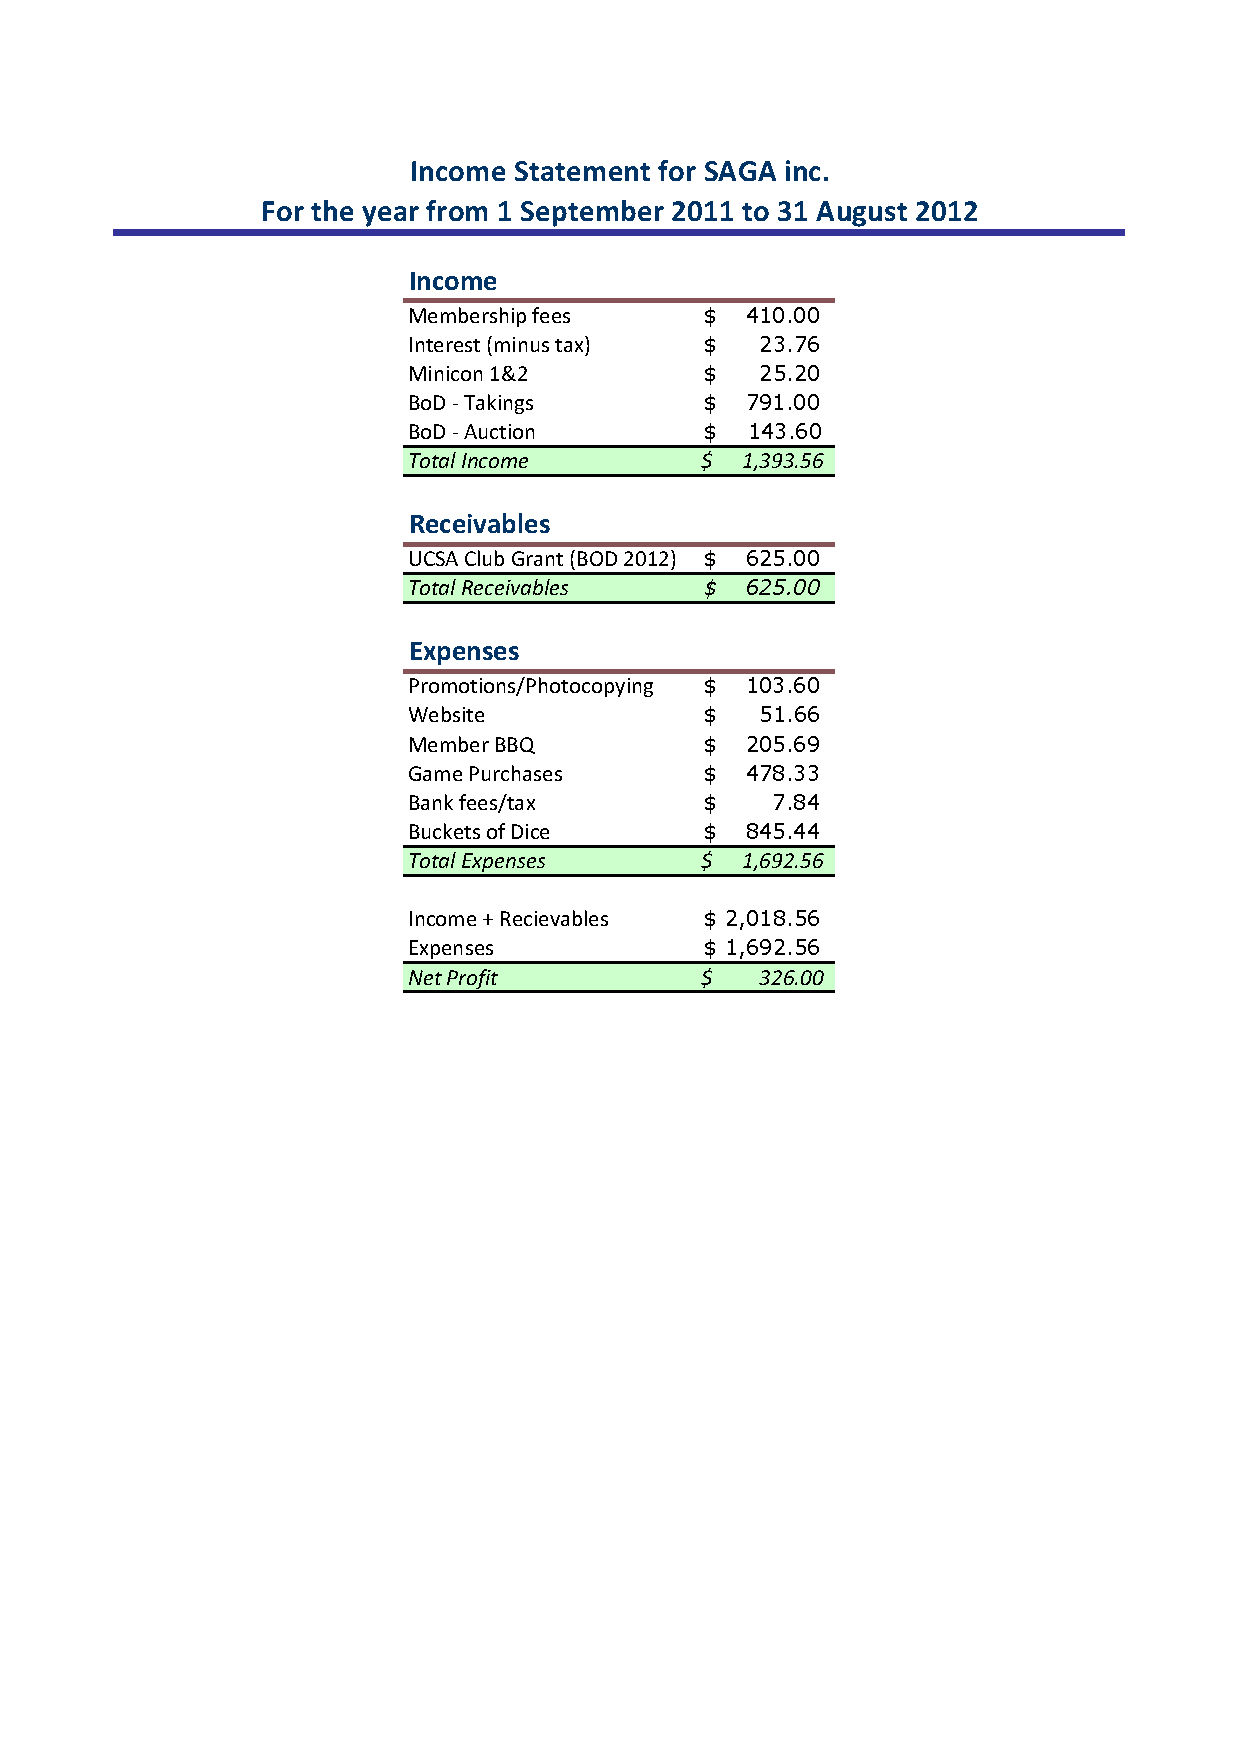
\includepdf{images/Income.pdf}
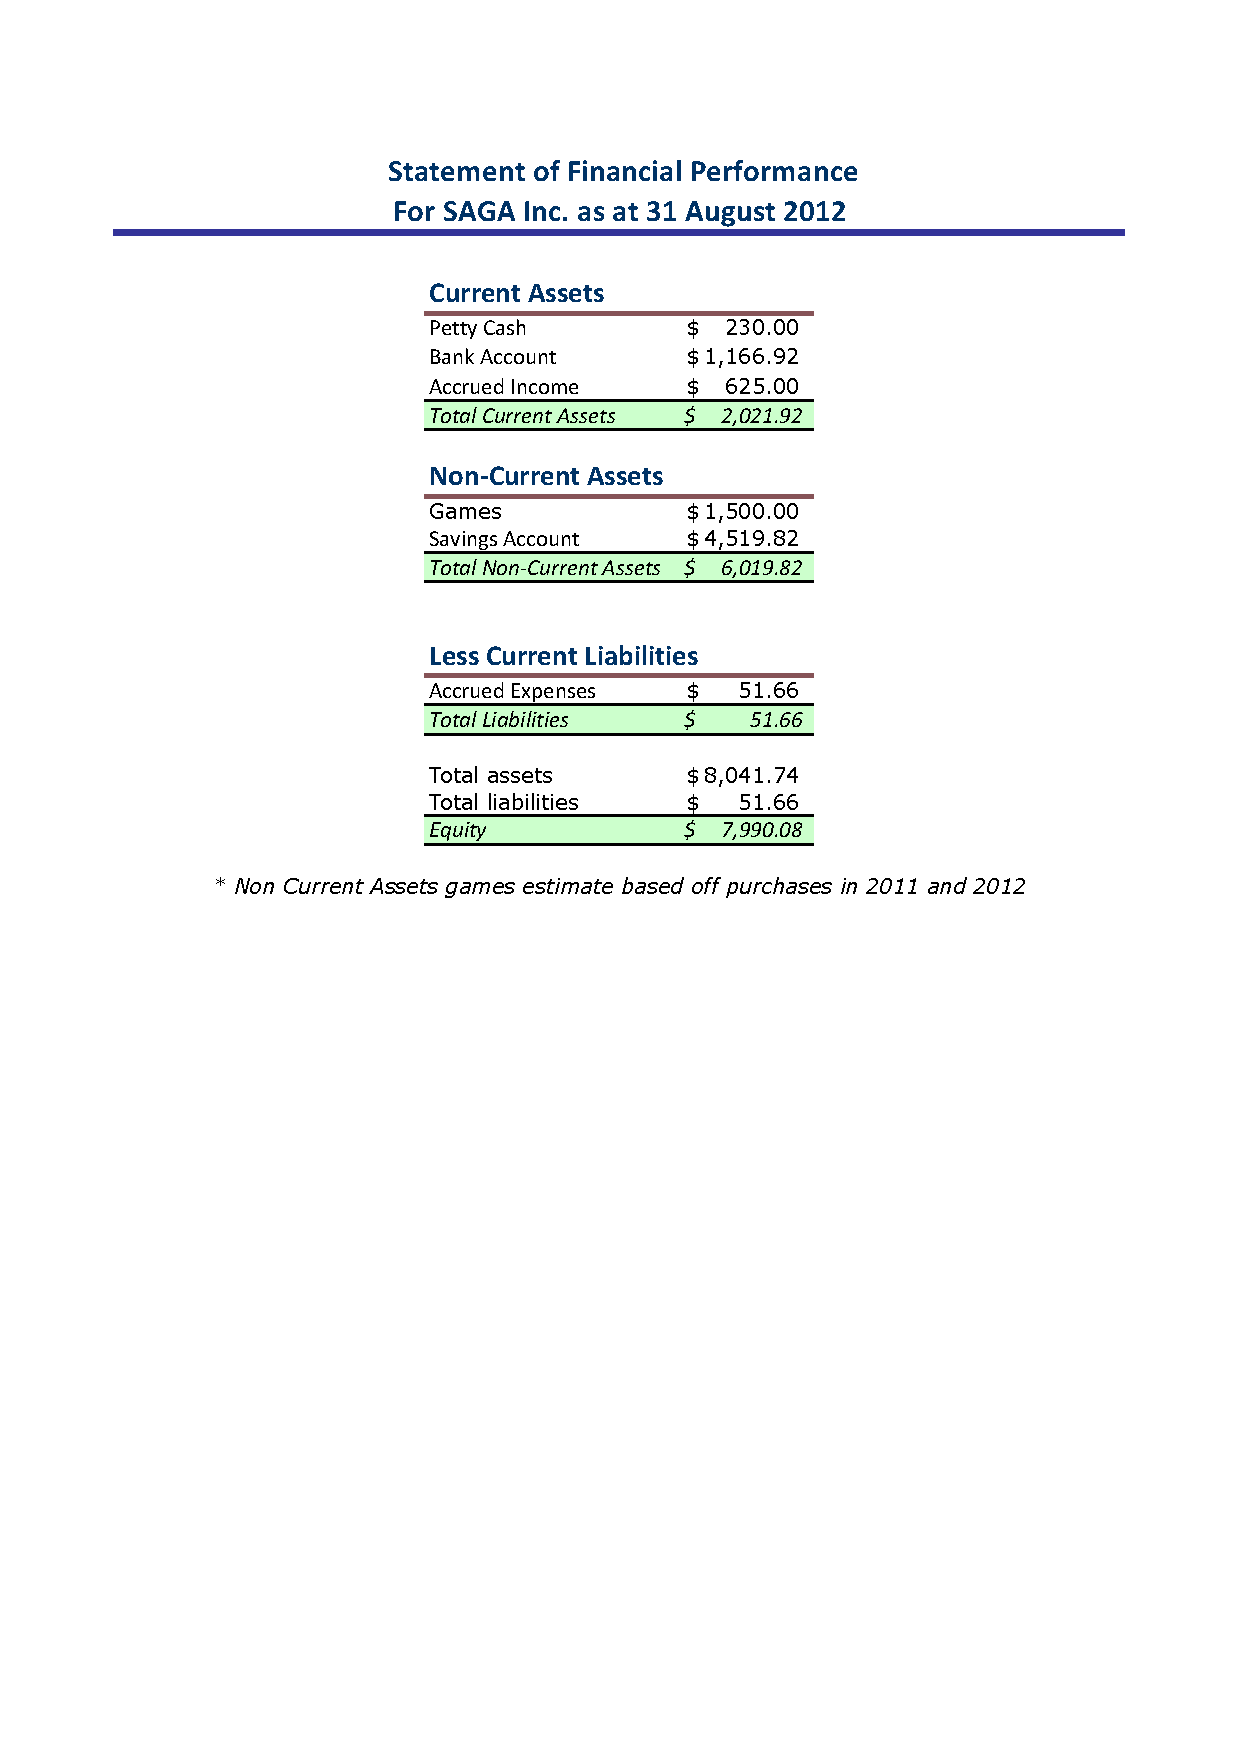
\includepdf{images/Financial.pdf}